\documentclass{homework}

\usepackage{graphicx}
\usepackage{subfig}
\usepackage{siunitx}

\title{Homework}
\author{Daniel Kadyrov}

\Title{Homework \#1}
\DueDate{February 11th, 2020}
\ClassName{Machine Learning}
\ClassNumber{CS559WS}
\ClassSection{Spring 2020}
\Instructor{Professor In Suk Jang}
\Author{Daniel Kadyrov}
\AuthorID{10455680}

\begin{document}

\maketitle

\begin{problem}[1]
    By using a change of variables, verify that the univariate Gaussian distribution given by:

    $$
    N(x \mid \mu , \sigma^2) = \frac{1}{\sqrt{2\pi\sigma^2}}\exp\{
        -\frac{1}{2\sigma^2}(x-\mu)^2
        \}
    $$

    satisfies $E(x) = \mu$. Next, by differentiating both sides of normalization condition

    $$
    \int_{-\infty}^{-\infty}N(x \mid \mu, \sigma^2) dx = 1
    $$

    with respect to $\sigma^2$, verify that the Gaussian satisfies $E(x^2)=\mu^2+\sigma^2$.
\end{problem}

\begin{solution}
    $$
    E(x) = \int_{-\infty}^{\infty} p(x|\mu, \sigma^2)x dx = E(x) = \int_{-\infty}^{\infty} \frac{x}{\sigma\sqrt{2\pi}}\exp\{-\frac{(x-\mu)^2}{2\sigma^2}\} dx
    $$
    $$
    E(x) = \int_{-\infty}^{\infty} \frac{x-\mu}{\sigma\sqrt{2\pi}}\exp\{-\frac{x^2}{2\sigma^2}\} dx
    $$

\end{solution}

\begin{problem}[2]
    Use $E(x) = \mu$ to prove $E(xx^T)=\mu\mu^T+\Sigma$. Now, using the results two definitions, show that:
    
    $$
    E[x_n x_m] = \mu\mu^T + I_{nm}\Sigma
    $$

    where $x_n$ denotes a data point same from a Gaussian distribution with mean $\mu$ and covariance $\Sigma$,and $I_{nm}$ denotes the $(n,m)$ element of the identity matrix. Hence prove the result (2.124)
\end{problem}

\begin{problem}[3]
    Consider a linear model of the form:

    $$
    f(x,w) = w_0 + \sum_{i=1}^D w_i x_i
    $$

    together with a sum of squares/loss function of the form:

    $$
    L_D(w) = \frac{1}{2} \sum_{n=1}^{N} (f(x_n,w)-y_n)^2
    $$

    Now suppose that Gaussian noise $\epsilon_i$ with zero mean and variance $\sigma^2$ is added independently to each of the input variables $x_i$. By making use of $E[\epsilon_i]=0$ and $E[\epsilon_i \epsilon_j]=\delta_{ij}\sigma^2$, show that minimizing $L_D$ averaged over the noise distribution is equivalent to minimizing the sum of square error for noise-free input variables with the addition of a weight-decay regularization term, in which the bias parameters $w_0$ is omitted from the regularizer.
\end{problem}

\newpage
\begin{problem}[4]
    \textbf{UCI Machine Learning: Bike Sharing Data Set}\\
    Build at least four regression models (e.g., linear, polynomial, non-linear) to predict the count of total rental bikes including both casual and registered. Explore data to reduce the number of features. Use K-fold cross validation and report the mean squared error (MSE) on the testing data. You need to write down every step in your experiment.
\end{problem}

\begin{solution}

The necessary packages and files are imported into the Python script: 

\begin{lstlisting}[language=Python]
import pandas as pd
from matplotlib import pyplot as plt
from sklearn.linear_model import LinearRegression, Ridge, Lasso, BayesianRidge
from sklearn.model_selection import KFold
from sklearn.metrics import mean_squared_error
import numpy as np

hour = pd.read_csv("hour.csv")
day = pd.read_csv("day.csv")

cnt_hour = hour["cnt"].values.reshape(-1, 1)
cnt_day = day["cnt"].values.reshape(-1, 1)
\end{lstlisting}

The data is explored to examine it's features. Both hourly and daily rider data is examined. The graphs outputted for the daily and hourly ridership are shown on the next pages, respectively. 

\begin{lstlisting}[language=Python]
for col in range(len(hour.columns)):
    if hour.columns[col] not in ["instant", "cnt", "dteday", "registered", "casual"]:
        plt.figure()
        plt.scatter(hour[hour.columns[col]].values.reshape(-1, 1), cnt_hour)
        plt.title("{} vs. Total Rider Hourly Count".format(hour.columns[col]))
        plt.xlabel("{}".format(hour.columns[col]))
        plt.ylabel("{}".format("Total Rider Count"))
        plt.savefig("images/hour_{}.png".format(hour.columns[col]))
        plt.clf()

for col in range(len(day.columns)):
    if day.columns[col] not in ["instant", "cnt", "dteday", "registered", "casual"]:
        plt.figure()
        plt.scatter(day[day.columns[col]].values.reshape(-1, 1), cnt_day)
        plt.title("{} vs. Total Rider Daily Count".format(day.columns[col]))
        plt.xlabel("{}".format(day.columns[col]))
        plt.ylabel("{}".format("Total Rider Count"))
        plt.legend()
        plt.savefig("images/day_{}.png".format(day.columns[col]))
        plt.clf()
\end{lstlisting}

\newpage
\begin{figure}[h]
\centering
\begin{subfigure} 
    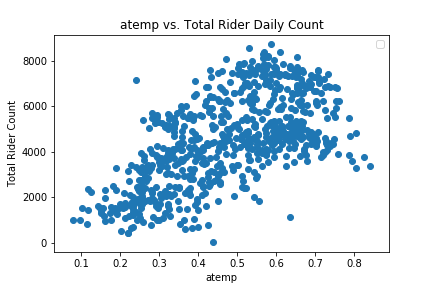
\includegraphics[width=50mm]{Bike-Sharing-Dataset/images/day_atemp.png}
\end{subfigure}
\begin{subfigure} 
    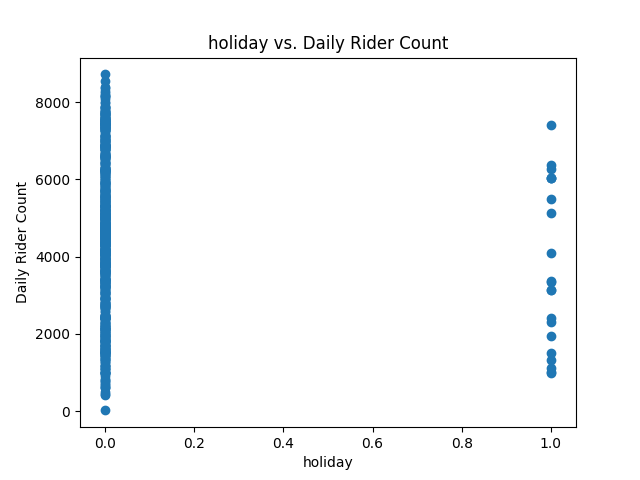
\includegraphics[width=50mm]{Bike-Sharing-Dataset/images/day_holiday.png}
\end{subfigure}
\begin{subfigure} 
    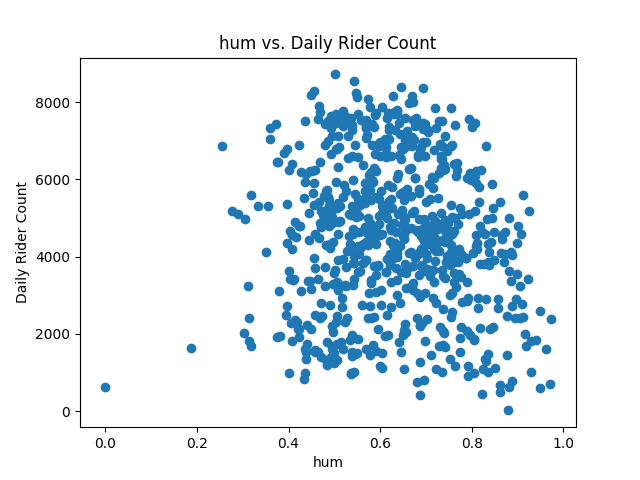
\includegraphics[width=50mm]{Bike-Sharing-Dataset/images/day_hum.png}
\end{subfigure}
\begin{subfigure} 
    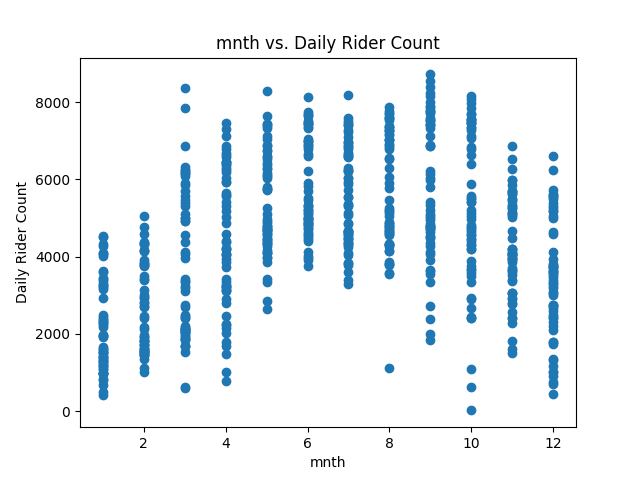
\includegraphics[width=50mm]{Bike-Sharing-Dataset/images/day_mnth.png}
\end{subfigure}
\begin{subfigure} 
    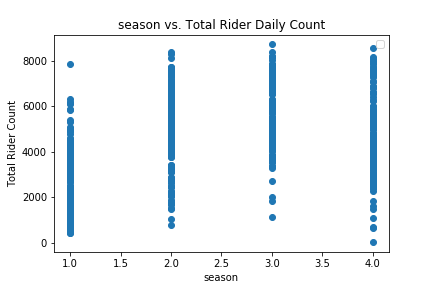
\includegraphics[width=50mm]{Bike-Sharing-Dataset/images/day_season.png}
\end{subfigure}
\begin{subfigure} 
    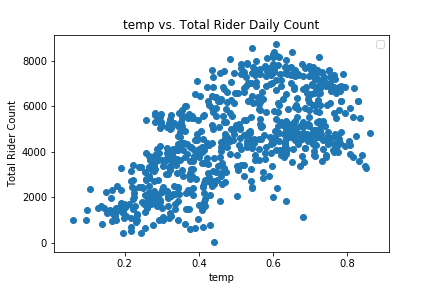
\includegraphics[width=50mm]{Bike-Sharing-Dataset/images/day_temp.png}
\end{subfigure}
\begin{subfigure} 
    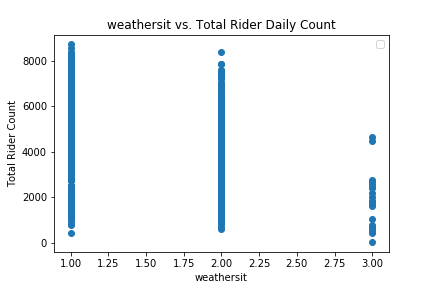
\includegraphics[width=50mm]{Bike-Sharing-Dataset/images/day_weathersit.png}
\end{subfigure}
\begin{subfigure} 
    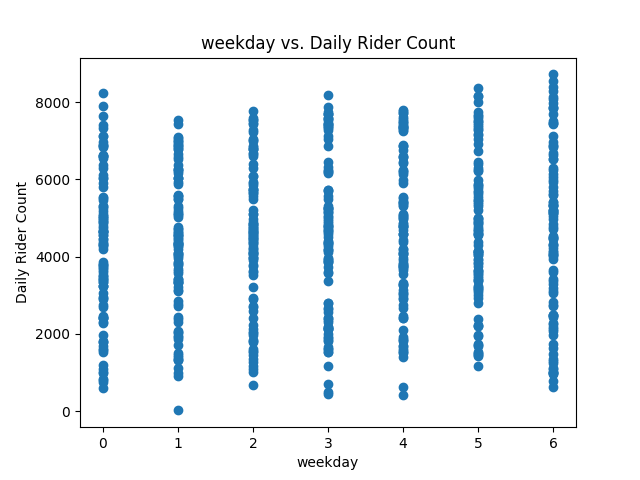
\includegraphics[width=50mm]{Bike-Sharing-Dataset/images/day_weekday.png}
\end{subfigure}
\begin{subfigure} 
    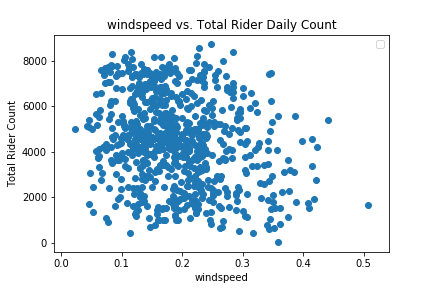
\includegraphics[width=50mm]{Bike-Sharing-Dataset/images/day_windspeed.png}
\end{subfigure}
\begin{subfigure} 
    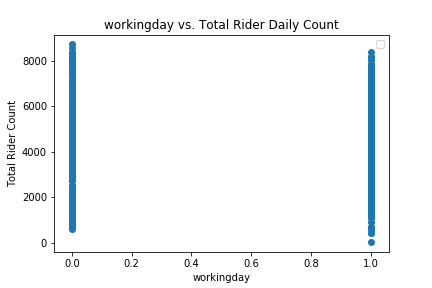
\includegraphics[width=50mm]{Bike-Sharing-Dataset/images/day_workingday.png}
\end{subfigure}
\begin{subfigure} 
    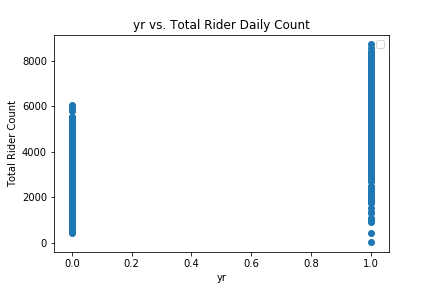
\includegraphics[width=50mm]{Bike-Sharing-Dataset/images/day_yr.png}
\end{subfigure}
\end{figure}

\newpage
\begin{figure}[h]
\centering
\begin{subfigure} 
    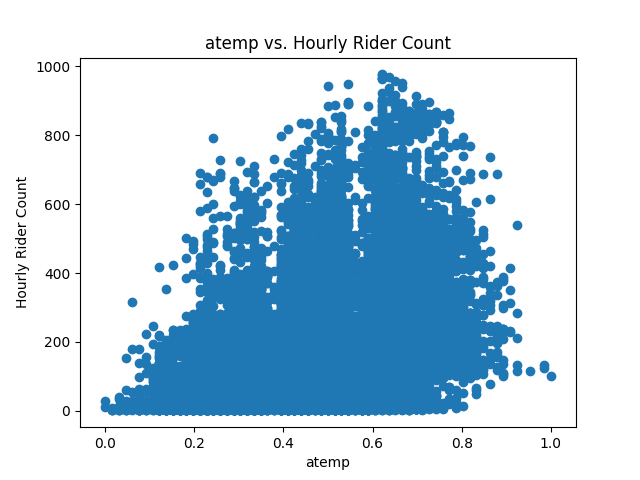
\includegraphics[width=50mm]{Bike-Sharing-Dataset/images/hour_atemp.png}
\end{subfigure}
\begin{subfigure} 
    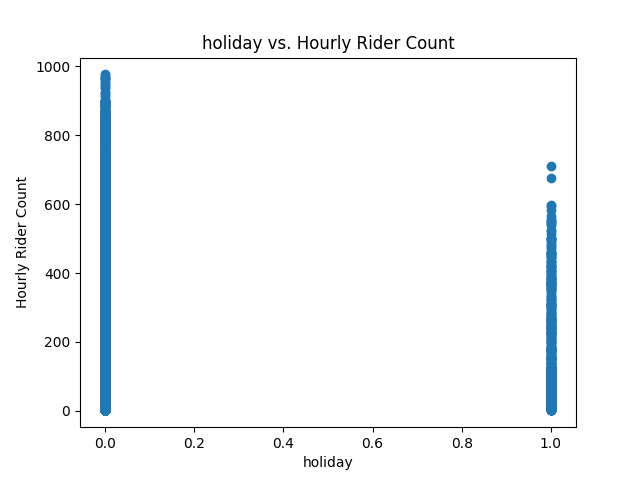
\includegraphics[width=50mm]{Bike-Sharing-Dataset/images/hour_holiday.png}
\end{subfigure}
\begin{subfigure} 
    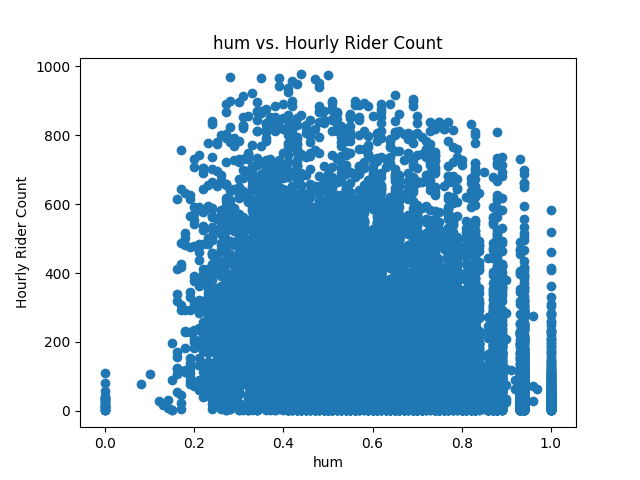
\includegraphics[width=50mm]{Bike-Sharing-Dataset/images/hour_hum.png}
\end{subfigure}
\begin{subfigure} 
    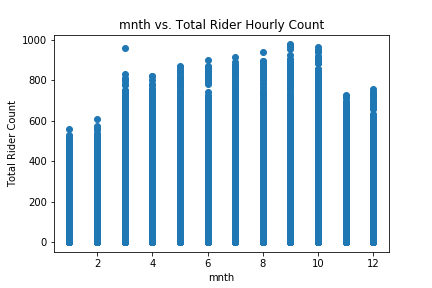
\includegraphics[width=50mm]{Bike-Sharing-Dataset/images/hour_mnth.png}
\end{subfigure}
\begin{subfigure} 
    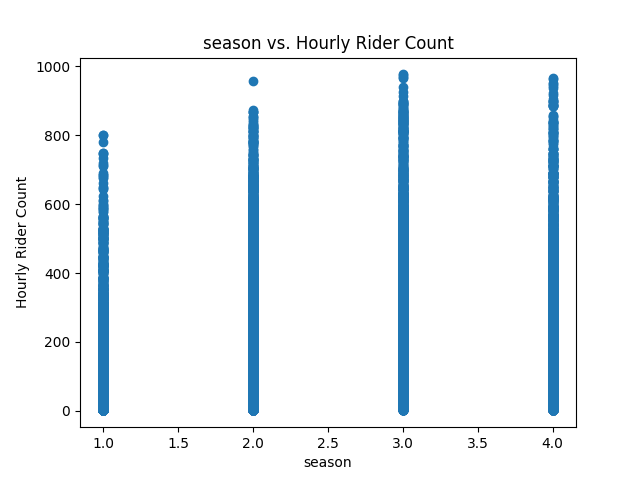
\includegraphics[width=50mm]{Bike-Sharing-Dataset/images/hour_season.png}
\end{subfigure}
\begin{subfigure} 
    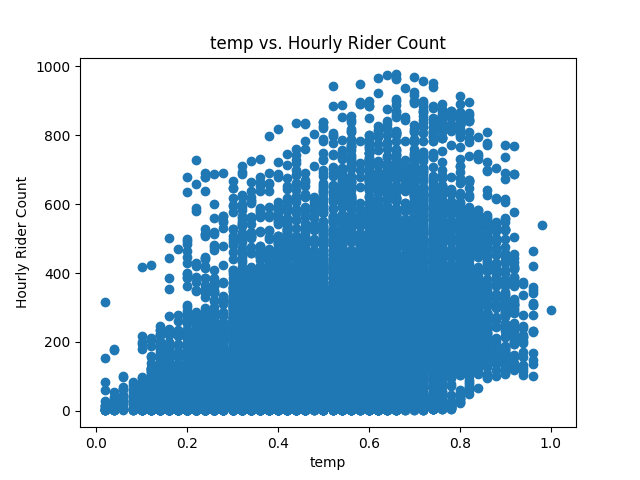
\includegraphics[width=50mm]{Bike-Sharing-Dataset/images/hour_temp.png}
\end{subfigure}
\begin{subfigure} 
    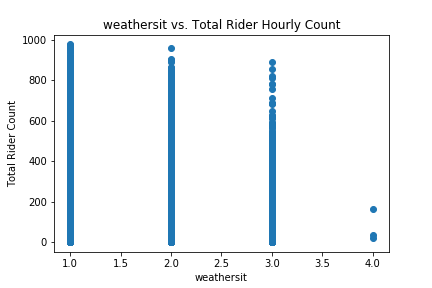
\includegraphics[width=50mm]{Bike-Sharing-Dataset/images/hour_weathersit.png}
\end{subfigure}
\begin{subfigure} 
    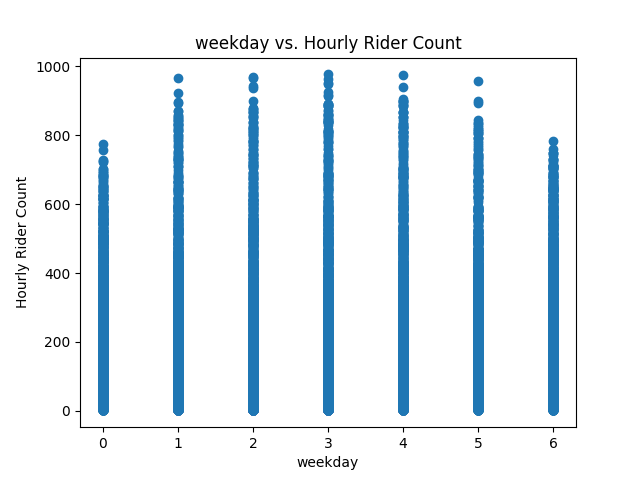
\includegraphics[width=50mm]{Bike-Sharing-Dataset/images/hour_weekday.png}
\end{subfigure}
\begin{subfigure} 
    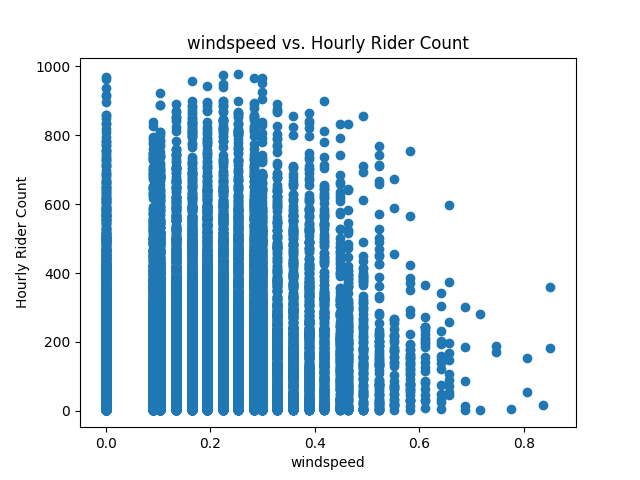
\includegraphics[width=50mm]{Bike-Sharing-Dataset/images/hour_windspeed.png}
\end{subfigure}
\begin{subfigure} 
    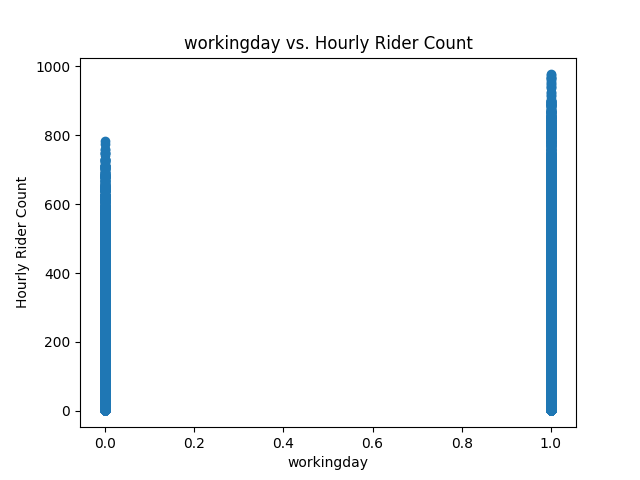
\includegraphics[width=50mm]{Bike-Sharing-Dataset/images/hour_workingday.png}
\end{subfigure}
\begin{subfigure} 
    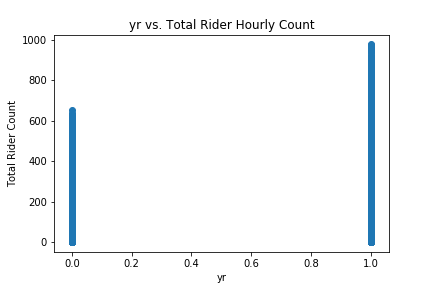
\includegraphics[width=50mm]{Bike-Sharing-Dataset/images/hour_yr.png}
\end{subfigure}
\end{figure}

\newpage
Based on the feature graphs, temperature was reduced to the best feature to model. According to the \texttt{README} the temperature was normalized with a \SI{41}{\celsius} maximum so the temperature array is multiplied by 41 for human readability. 

\begin{lstlisting}
day_temp = day["temp"].values.reshape(-1, 1) * 41
\end{lstlisting}

KFold cross-validation was used with a 10-split. The regression models applied were linear, ridge, lasso, and bayesian through their respective \texttt{sklearn} packages. For each k-fold, the models are fitted using the separated training data. 

\begin{lstlisting}
crossvalidation = KFold(n_splits=10)
linear = LinearRegression()
ridge = Ridge()
lasso = Lasso()
bayesian = BayesianRidge()

for train_index, test_index in crossvalidation.split(day_temp):
    X_train, X_test = day_temp[train_index], day_temp[test_index]
    y_train, y_test = cnt_day[train_index], cnt_day[test_index]
    linear.fit(X_train, y_train)
    ridge.fit(X_train, y_train)
    lasso.fit(X_train, y_train)
\end{lstlisting}

The test portion of the data was then used to test the prediction quality of the models. The mean square error was calculated between the test portion data and the values predicted by the models. 

\begin{lstlisting}
linear_pred = linear.predict(X_test)
ridge_pred = ridge.predict(X_test)
lasso_pred = lasso.predict(X_test)
bayesian_pred = bayesian.predict(X_test)

mse_linear = mean_squared_error(y_test, linear_pred)
mse_ridge = mean_squared_error(y_test, ridge_pred)
mse_lasso = mean_squared_error(y_test, lasso_pred)
mse_bayesian = mean_squared_error(y_test, bayesian_pred)
\end{lstlisting}

The following a table showing the different mean squared error values of the models. 

\begin{table}[h]
    \centering
    \begin{tabular}{|l|l|}
    \hline
    Model  & Mean Squared Error \\ \hline
    Linear & 4306257.419012716 \\ 
    Ridge  & 4306194.805960745 \\ 
    Lasso  & 4306018.563140404 \\ 
    Bayesian & 4301889.80709847 \\
    \hline
    \end{tabular}
    \end{table}

    \begin{figure}[h]
        \centering
        \begin{subfigure} 
            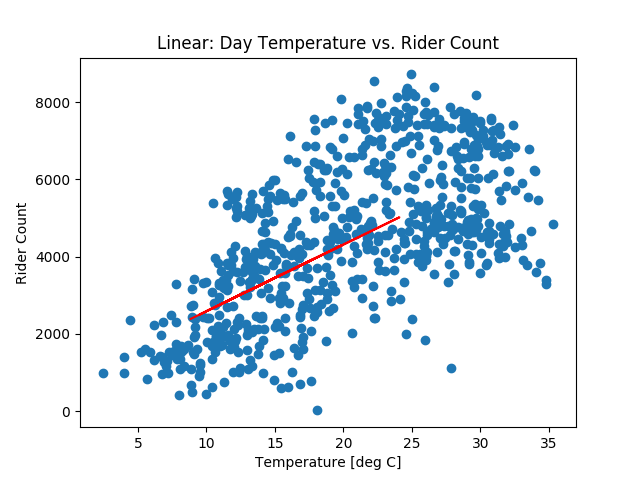
\includegraphics[width=75mm]{Bike-Sharing-Dataset/images/linear.png}
        \end{subfigure}
        \begin{subfigure} 
            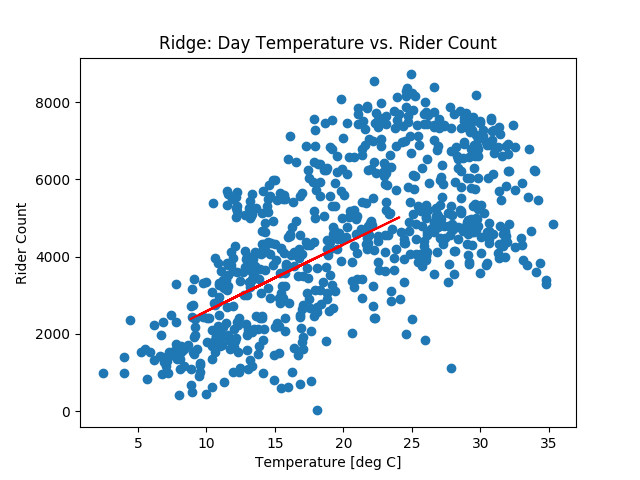
\includegraphics[width=75mm]{Bike-Sharing-Dataset/images/ridge.png}
        \end{subfigure}
        \begin{subfigure} 
            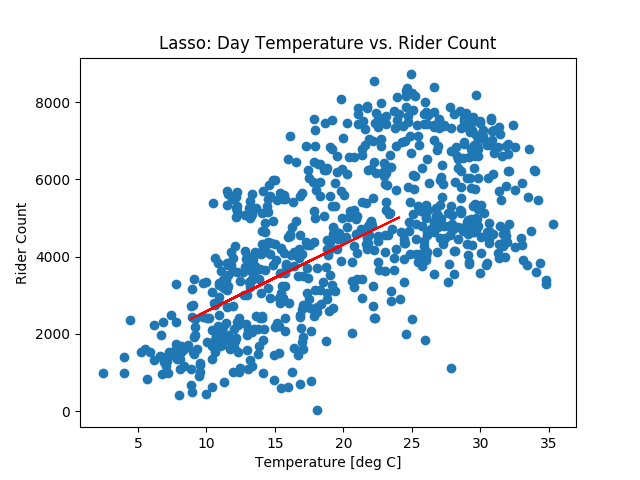
\includegraphics[width=75mm]{Bike-Sharing-Dataset/images/lasso.png}
        \end{subfigure}
        \begin{subfigure} 
            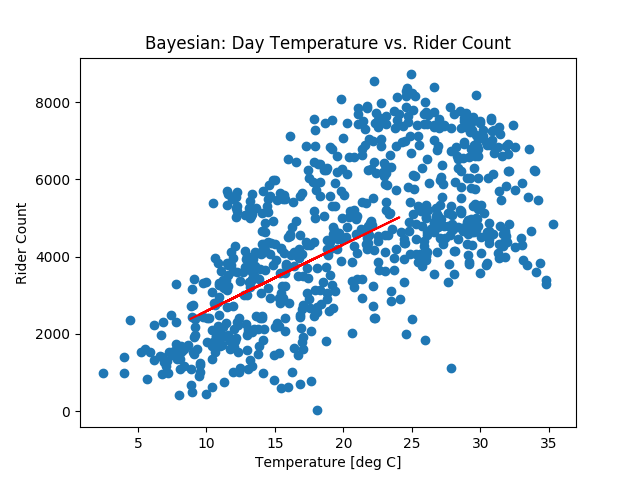
\includegraphics[width=75mm]{Bike-Sharing-Dataset/images/bayesian.png}
        \end{subfigure}
        \end{figure}

\end{solution}

\end{document}